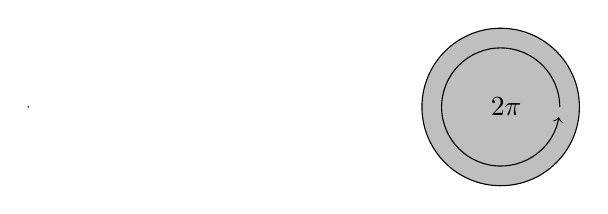
\begin{tikzpicture}
\draw (0,0) circle (0.0001cm);
\filldraw[draw = black, fill = lightgray] (6,0) circle (1cm);
\draw[->] (6.75,0) arc(0:350:0.75);
\draw (5.75,0) node[anchor=west] {$2\pi$};
\end{tikzpicture}
\newline

It can often be hard for people to learn about angular velocity because we see things spinning a lot less than we see them moving linearly. Up until now, we have only considered things moving around in space, but things can also spin. As we will see, there are many parallels between linear and rotational motion. The first thing we want to do is define angular velocity. Angular velocity will be a measure of how fast an object(perhaps a fidget spinner, or a disk), is rotating about a certain axis. Often the axis will be the center of the object, but it does not have to be. For our purposes, let us imagine that we have a disk rotating around its center, similar to how a fan spins. We can think about what happens during one time that it spins around. We say that in one revolution, the wheel would have spun around $360^o$. In radians, this corresponds to $2\pi$ radians. However, one weird thing about angular motion is that when an object has undergone a $2\pi$ radian movement, so it is essentially in the same position as before. If it went around again, we would say it has gone around $4\pi$ radians. This would not, however, be the case if we spun an object $2\pi$ radians clockwise, and then spun it counterclockwise. In that case, we would say the object had experienced a 0-radian angle change. So, essentially, even though either way the object looks the same before and after, we have a different change in the angle. This will be very important when talking about objects that might rotate thousands of times per second. However, we can also think about the rate at which the wheel is spinning. After all, a rotating disk will be of little use if it takes ten years before it can spin around one time. The rate at which a disk(or any rigid body for that matter), spins is called its angular velocity, $\omega$. A larger $\omega$ will correspond to the disk rotating around faster while a smaller $\omega$ corresponds to the disk rotating around more slowly. $\omega$ is defined as the number of radians that a point on a rigid body will move in one second. We can also define it in the same way as we defined linear velocity, as an angular displacement divided by a change in time. $$\frac{\Delta \theta}{\Delta t}$$ An angular displacement will be a slight change in the angle of the spinning object. So the object might turn a little bit. As you have probably seen plenty of times by now, we can take the limit of this equation to find that $$\frac{\Delta \theta}{\Delta t}$$ as $t$ goes to 0. We find that the instantaneous angular velocity is \begin{equation}\omega=\frac{d\theta}{dt}\end{equation} $\omega$ is called omega. This quantity will be in the units of radians per second. However, we do not consider radians in any practical matters(essentially we will pretend as if rads/second is just 1/seconds). Rigid bodies will have the same $\omega$ for all points on their surface by definition. This may seem odd, but you have to remember that angular velocity is only considered with rotation about an angle, and not necessarily about the true distance a point might be traveling. These definitions might have seemed kind of vague, but you will in time see that the idea is quite simple. Also, you will note that because $\omega$ is the same for all points on a rigid body, we will generally talk about the rotation of the whole body rather than the rotation of a specific point. 

Imagine we have a frisbee rotating about the top of my finger off of the center of the frisbee. Every $n$ seconds, the frisbee completes an entire rotation about the center of the frisbee. A rotation corresponds to an angular displacement of $2\pi$ radians. So the angular velocity is $$\frac{2\pi}{n} \frac{radians}{second}$$ using Eqn. 6.1.1. So moving every $\frac{2\pi}{n}$ radians takes 1 second for the frisbee to complete. Of course, closely related to the angular velocity is angular acceleration, which is much less intuitive but very important. Essentially, like acceleration, angular acceleration (symbolized by $\alpha$, pronounced alpha)  measures the change in angular velocity of a spinning object rather than a linearly moving object. It is defined as either $$\frac{d\omega}{dt}$$(for instantaneous acceleration), $$\frac{\Delta \omega}{\Delta t}$$(for average acceleration), or $$\frac{d^2\theta}{dt^2}$$ All three of these definitions can prove useful at the right times. Now, let us do a simple and contrived example to display angular acceleration. Say that an object is experiencing an angular velocity $\omega \left(t\right)$ that is changing as a function of time with $$\omega \left(t\right)=kt \frac{radians}{second}$$ We know that \begin{equation}\frac{d \omega}{dt}=\alpha\end{equation} so $\alpha=k$. This is a fairly boring question, a more interesting question might be, "by how many radians does the object rotate in time $t$?". To do this, we have to work from the angular velocity back to the angle by using integration, just like we did with linear velocity. We can say, as we did with the position, that the change in the angle of the object over a period is equal to the integral of the angular velocity of the object over the same time. So in our case the angular displacement is $$\int_{t_1}^{t_2} kt$$ is $$\frac{k\left(t_{2}^2-t_{1}^2\right)}{2}$$